\section{Introduction}

Neural networks have been successful in various natural language processing tasks,
where end-to-end training become a primary option \cite{Seo2016}.
As the design of neural networks evolve, there is a clear trend that more and more
parameters participate in training and prediction. While the strong expressivity
enhance model performance, the lack of interpretability presents challenge for analysis.
Without understanding the background meaning that features carry, visualization relies
on proper quantification analysis (cite). Such analysis is not easy to come up with,
and is tied to specific task (cite).

Recently attention networks become a widely-adopted setup (cite), partly because it yields
intermediate representations (e.g. alignment) that are not just beneficially expressive for performance,
but also intuitive to model. Indeed, the interpretability of attention networks introduce
a natural interface for analyzing the inside of neural networks. The wide popularity of attention networks
in recent NLP works necessitate a convenience framework for visualization and analyzing.

To facilitate exploration in attention models, we introduce an interactive visualization toolset
for word-attention models. We demonstrate our system on two primary NLP tasks: natural language
inference (NLI) and machine comprehension (MC). For the NLI task, we visualize
decomposable attention networks which represents a series of strongly performing models \cite{}.
For the MC task, we present your visualization methods on bidirectional attention flow model,
which also represents a line of strong models \cite{}.

\begin{figure}[htbp]
\centering
\vspace{-2mm}
 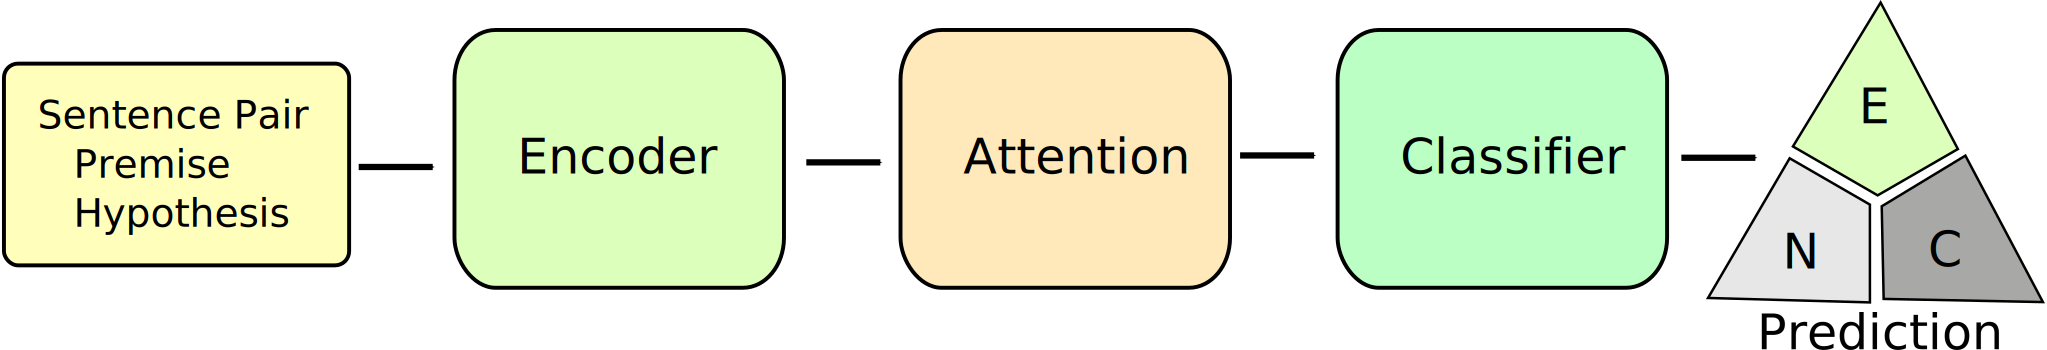
\includegraphics[width=1.0\linewidth]{pipeline}
 \caption{
 Perturbation-Driven Exploration of the NLP Model.
 }
\label{fig:modelPipeline}
\end{figure}


In summary, our key contributions are:
\begin{itemize}
	\item Introduce an flexible visualization system for creating customized interactive visual analytic environment for attention centric neural networks model in NLP. 
	\item Illustrate the importance of streamlining the query to the model
	\item Demonstrate our system on two major NLP tasks with strong-performing
	models. We observe functional limitations of these models which can be helpful
	for future improvement on modeling.
\end{itemize}


exploration task
\cite{Seo2016}
Comparsion with AllenNLP
